\newpage
\section{Punto 1}
\textit{Construir un algoritmo que permita, utilizando Hashing, resolver el siguiente problema: Dado el texto de un archivo, escrito en lenguaje coloquial, generar un listado de palabras diferentes y la cantidad de veces que aparece cada una en el texto.
}\\


El método implementado lee el texto que se encuentra en un archivo \path{.txt}, convierte los caracteres iniciales de cada palabra a minúsculas (asumiendo que no hay mayúsculas en la mitad de las palabras), toma palabra a palabra del texto y lo guarda en un arreglo para luego utilizar las palabras como key de la tabla hash, almacenando la cantidad de veces que dicha palabra aparece en el texto, cada vez que se intenta agregar una palabra, el valor que la tabla hash tiene almacenado para la key ``palabra'' incrementara en uno, en la figura \ref{fig:Consola hash palabra} se observa la salida resultante

\begin{figure}
  \centering
  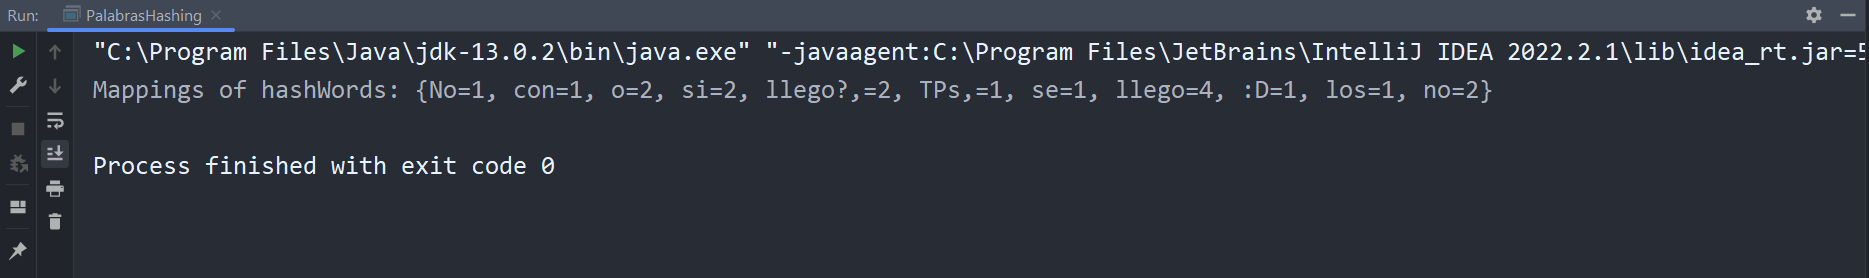
\includegraphics[width=\textwidth, scale=1]{Images/Punto3/ConsolaHashPalabra.png}
  \caption{Salida por consola para el texto \ref{lst:textoEntradaHash} }
  \label{fig:Consola hash palabra}
\end{figure}

\begin{lstlisting}[style=java, caption= Texto de entrada, label={lst:textoEntradaHash}]
  No se si llego con los TPs
  llego o no llego?
  llego o no llego?
  si llego :D
  
 \end{lstlisting}
 \label{fig:Traza ordenamiento por conteo}

 \begin{lstlisting}[style=java, caption= Metodo readAndHash()\cite{readAndHashMetodo}]
  public static void readAndHash(Hashtable<String,Integer> hashWords) throws IOException {
    String filePath = "src\\T1P2\\texto.txt";
    File file = new File(filePath);
    BufferedReader br = new BufferedReader(new FileReader(file));
    String st;
    String [] words =null;
    int lenghtArrayOfWords;

    while((st = br.readLine())!=null){//Continua mientras tenga lineas por leer, va linea por linea
      words = st.split(" "); //Genera array de palabras separadas por espacios
      Arrays.stream(words).map(word -> word.toLowerCase()); //Convierte a minusculas las mayusculas
      lenghtArrayOfWords = words.length;
      for (int i = 0; i < lenghtArrayOfWords; i++) {
        if(hashWords.containsKey(words[i])){
          hashWords.put(words[i], hashWords.get(words[i])+1);
        }else{
          hashWords.put(words[i],1);
        }
      }
    }
  }
 \end{lstlisting}